\chapter{References}
Miller, K.J., Adair, B.S., Pearce, A.J., Said, C.M., Ozanne, E. and Morris, M.M., 2014. Effectiveness and feasibility of virtual reality and gaming system use at home by older adults for enabling physical activity to improve health-related domains: a systematic review. Age and ageing, 43(2), pp.188-195. 

M. Slater and M. Usoh (1993) ’Presence in Immersive Virtual Environments’, - Proceedings of IEEE Virtual Reality Annual International Symposium, pp. 90. 

Roginska, A. and Geluso, P. (2017) Immersive Sound: The Art and Science of Binaural and Multi-Channel Audio: Taylor Francis. 

Rebenitsch, L., 2016. Review on cybersickness in applications and visual displays. [online] Available at: https://link.springer.com/article/10.1007%2Fs10055-016-0285-9 [Accessed 7 November 2021]. 

Slater, M., Lotto, B., Arnold, M.M. and S´anchez-Vives, M.V. (2009a) ’How we Experience Immersive Virtual Environments: The Concept of Presence and its Measurement’. Anuario De Psicolog´ıa, 2009, Vol.40, P.193-210, 


\chapter{Table of figures}

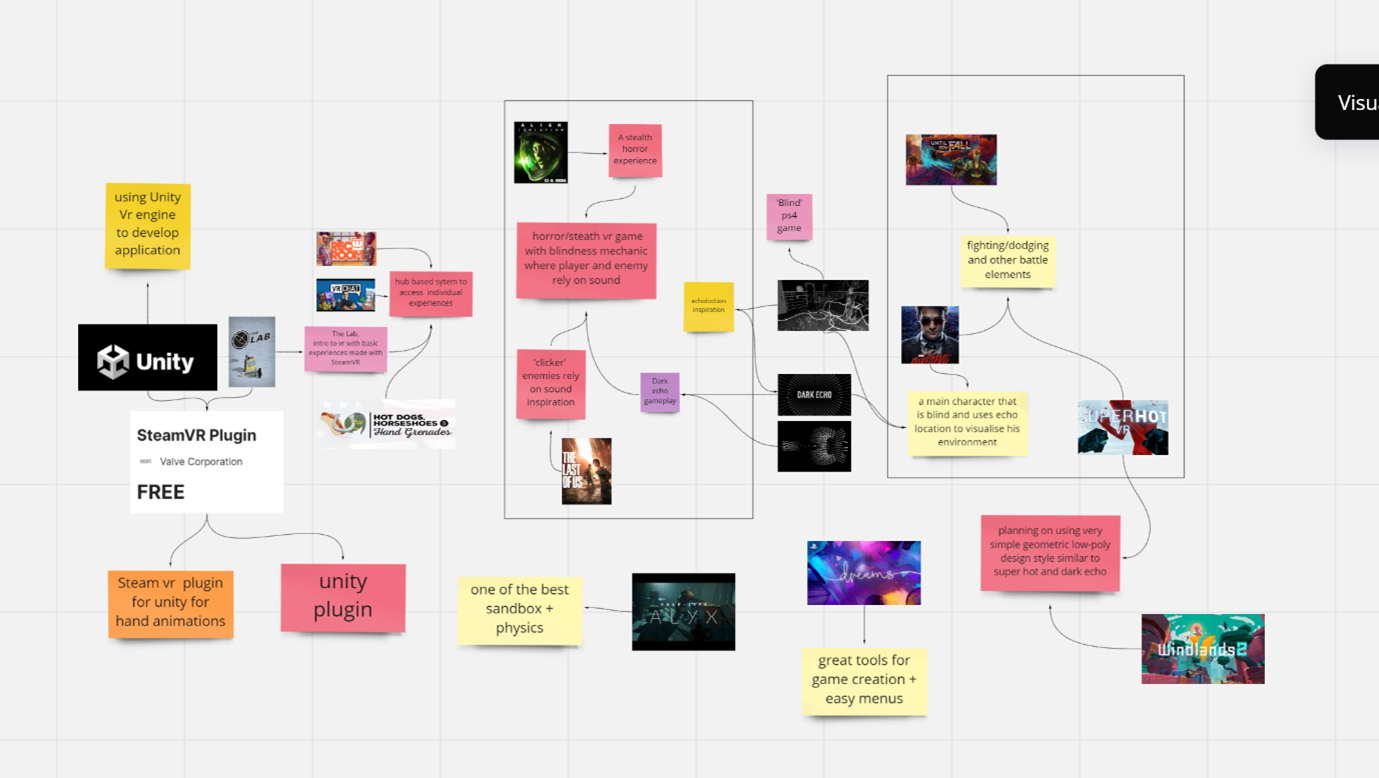
\includegraphics[width=15cm]{Chapters/Picture1.png}

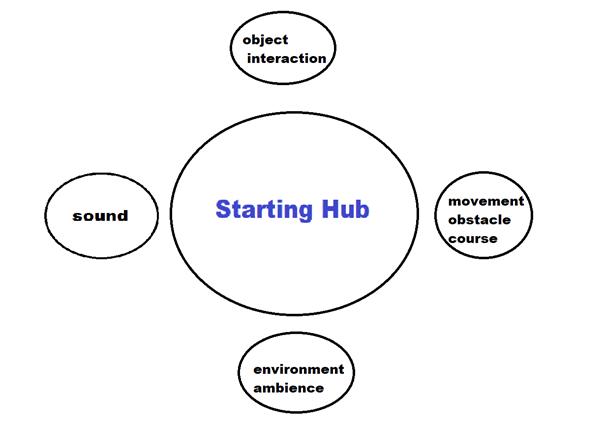
\includegraphics[width=15cm]{Chapters/Picture2.png}

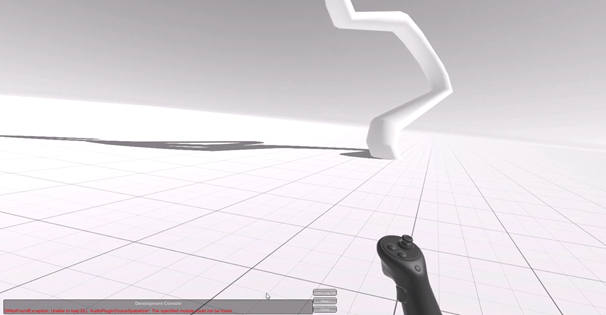
\includegraphics[width=15cm]{Chapters/Picture3.png}

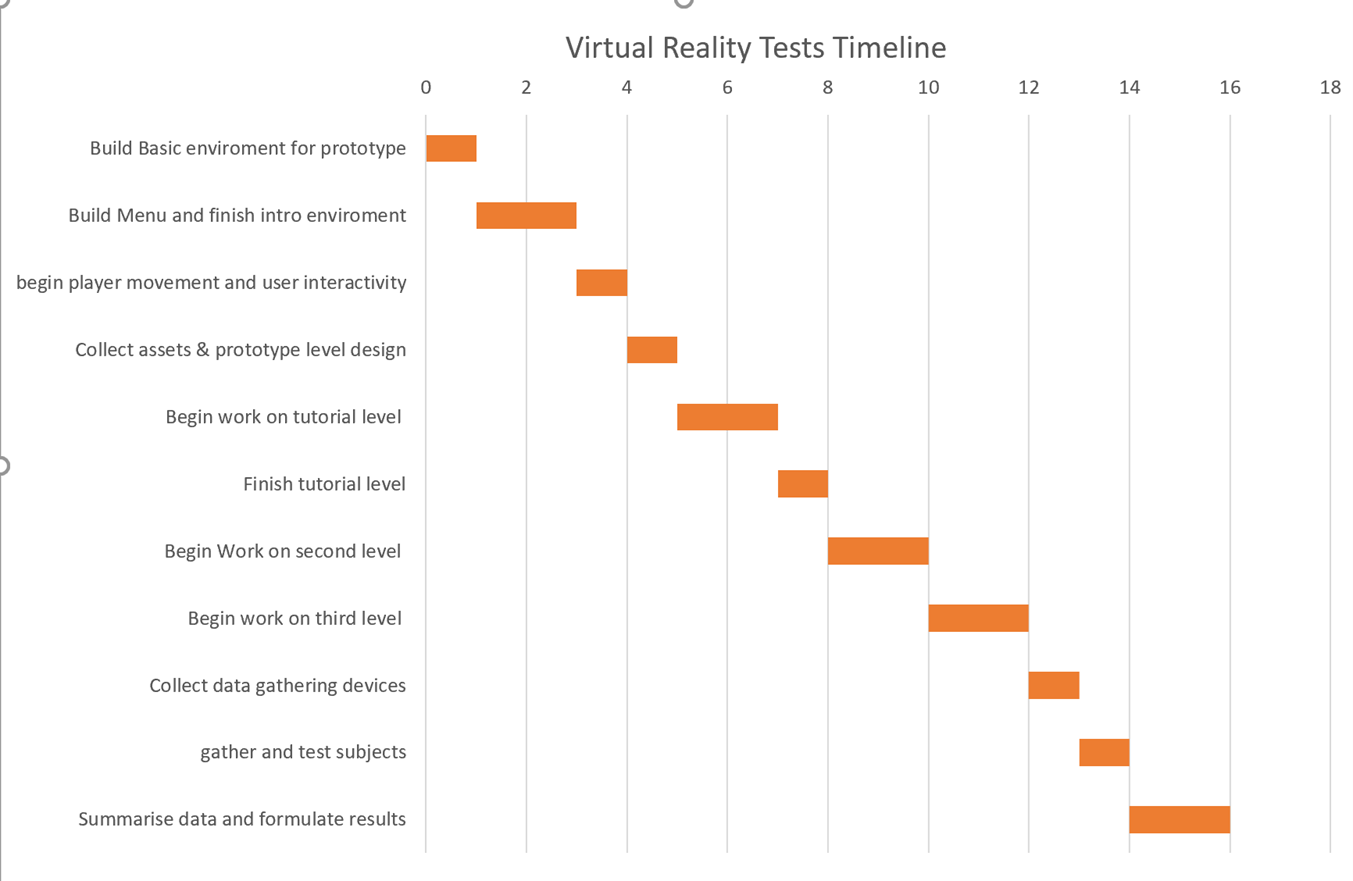
\includegraphics[width=15cm]{Chapters/Picture4.png}